\subsection{Model Parameter Analysis}

An important consideration when comparing neural network architectures is the number of trainable parameters, which directly impacts model complexity, memory requirements, and computational demands. We analyzed the parameter counts for each model architecture with both single-neuron and dual-neuron output configurations.

\begin{figure}[htbp]
\centering
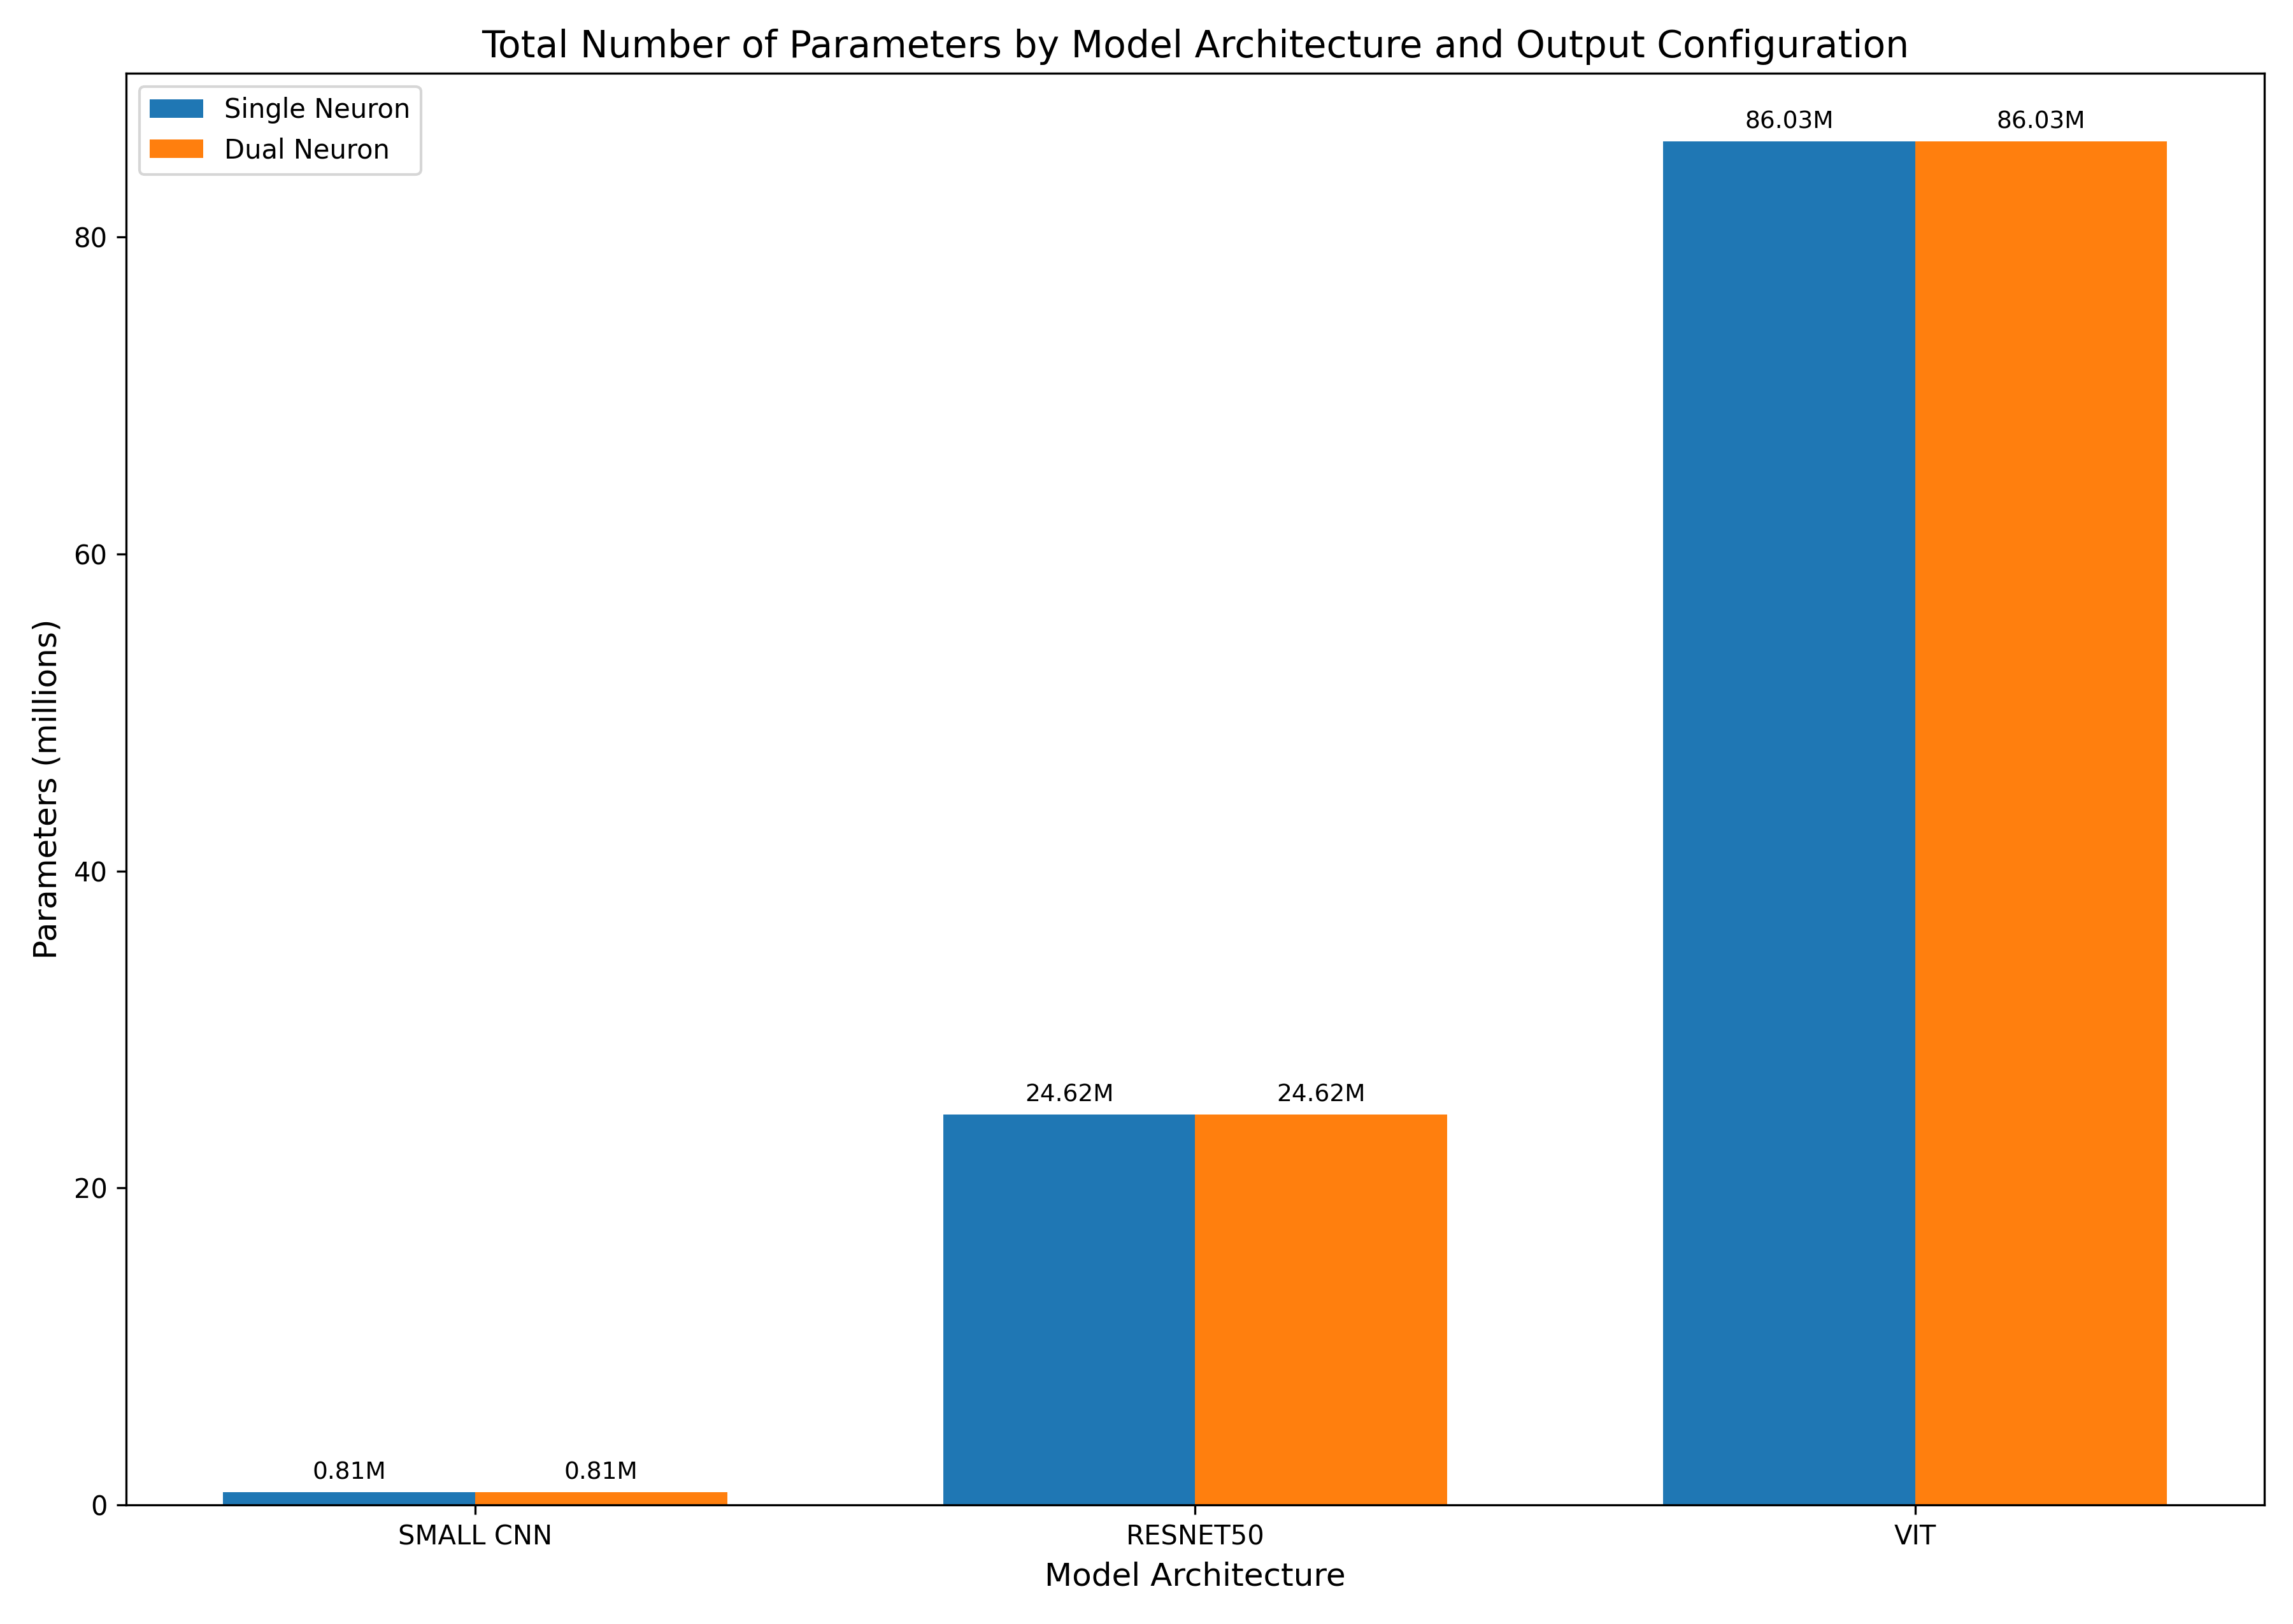
\includegraphics[width=\textwidth]{figures/parameter_count_comparison.png}
\caption{Comparison of trainable parameter counts across model architectures with single-neuron and dual-neuron output layers. The difference between configurations is minimal relative to total parameter count.}
\end{figure}

The figure above illustrates the total parameter counts (both trainable and non-trainable) for each architecture. The Vision Transformer (ViT) has the highest parameter count (approximately 86 million parameters), followed by ResNet50 (approximately 25 million parameters), and finally the Small CNN (approximately 813,000 parameters). This reflects the inherent complexity of these architectures, with ViT's attention mechanisms requiring significantly more parameters than traditional convolutional approaches.

Table~1 provides a detailed breakdown of the parameter counts for each architecture with both output configurations:

\begin{table}[htbp]
\centering
\begin{tabular}{lccc}
\hline
\textbf{Architecture} & \textbf{Output Type} & \textbf{Total Parameters (M)} & \textbf{Trainable Parameters (M)} \\
\hline
Small CNN & Single Neuron & 0.81 & 0.81 \\
Small CNN & Dual Neuron & 0.81 & 0.81 \\
\hline
ResNet50 & Single Neuron & 24.62 & 16.08 \\
ResNet50 & Dual Neuron & 24.62 & 16.08 \\
\hline
Vision Transformer & Single Neuron & 86.03 & 0.23 \\
Vision Transformer & Dual Neuron & 86.03 & 0.23 \\
\hline
\end{tabular}
\caption{Parameter counts for each model architecture with single-neuron and dual-neuron output configurations. Values are shown in millions (M) of parameters.}
\label{tab:parameter_counts}
\end{table}

As shown in the table, the difference in parameter count between single-neuron and dual-neuron configurations is remarkably small for all architectures:

\begin{enumerate}
\item \textbf{Small CNN}: The dual-neuron configuration adds only 257 additional parameters (0.03\% increase) compared to the single-neuron model.

\item \textbf{ResNet50}: The dual-neuron configuration adds only 129 additional parameters (0.0008\% increase).

\item \textbf{Vision Transformer}: The dual-neuron configuration adds only 129 additional parameters (0.06\% increase).
\end{enumerate}

\begin{figure}[htbp]
\centering
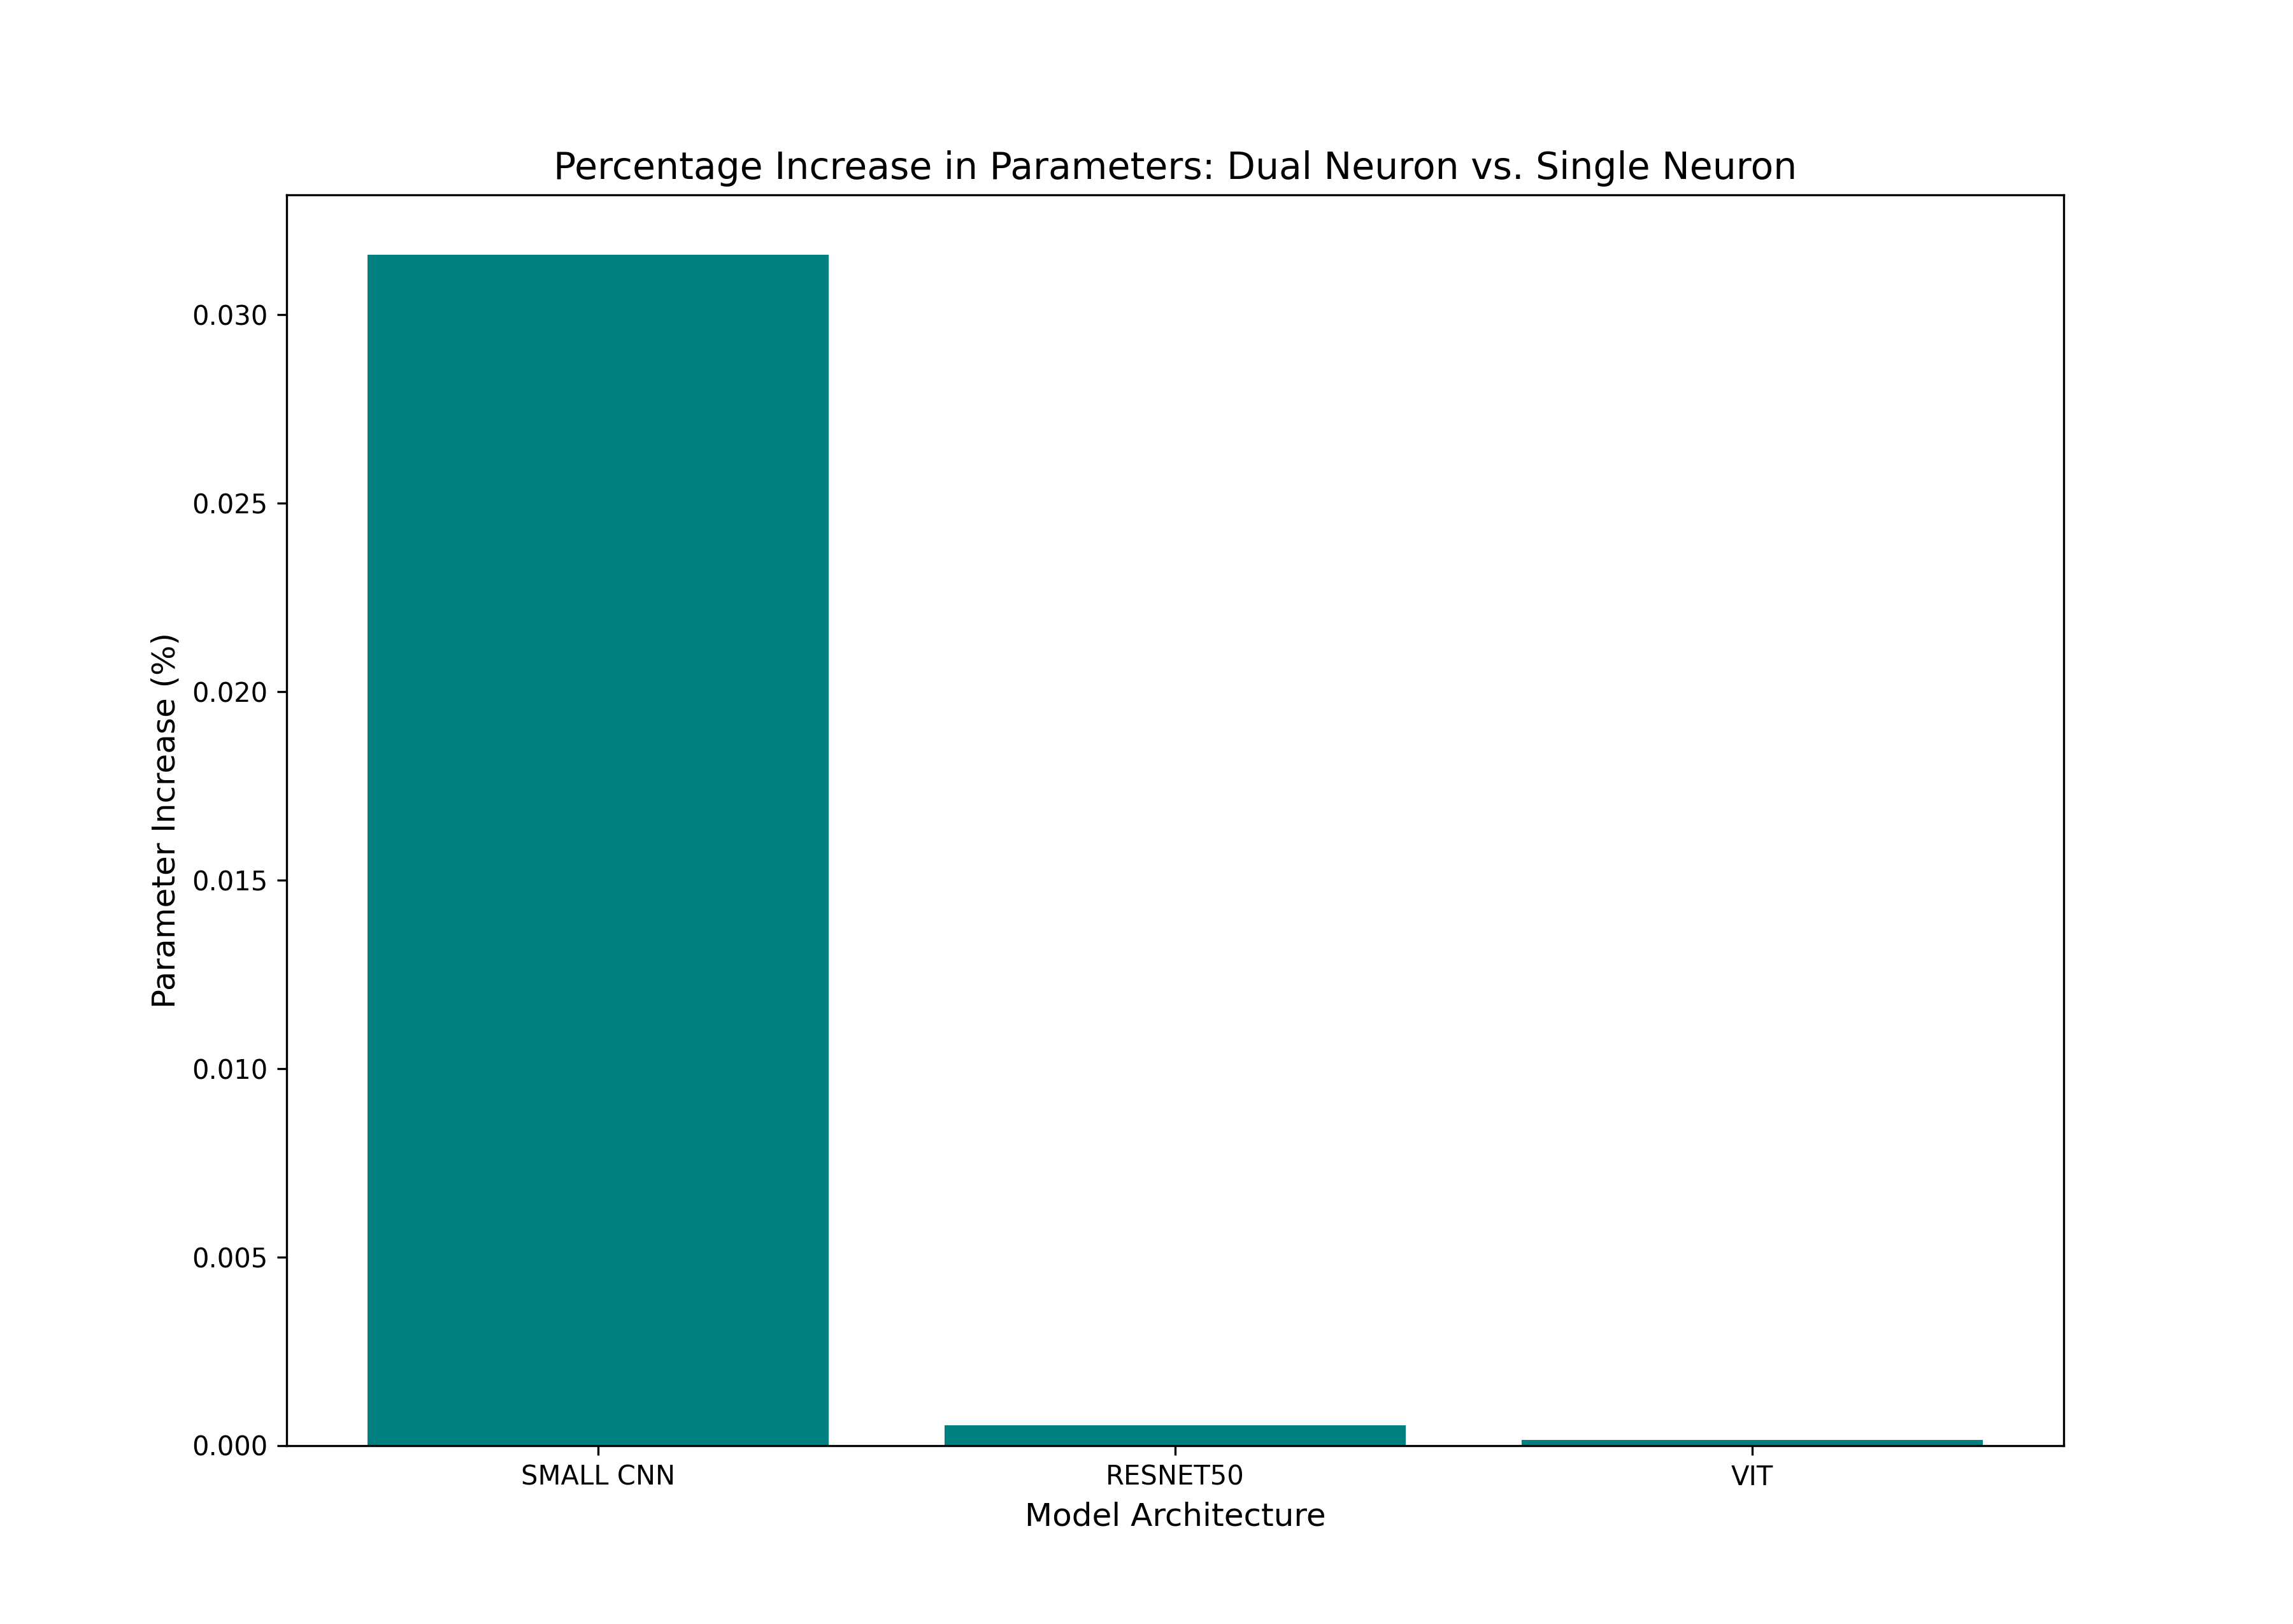
\includegraphics[width=\textwidth]{figures/parameter_increase_percentage.png}
\caption{Percentage increase in parameters when using dual-neuron output layer compared to single-neuron configuration. The increase is negligible across all architectures.}
\end{figure}

The second figure shows the percentage increase in parameters when switching from a single-neuron to a dual-neuron output layer. This analysis reveals that the parameter count difference between the two approaches is negligible relative to the total model size, with increases of less than 0.1\% across all architectures.

This finding is significant because it demonstrates that the performance differences observed between single-neuron and dual-neuron configurations cannot be attributed to model capacity or complexity. It's worth noting that while ViT has the highest total parameter count, most of these parameters are frozen during training as part of our transfer learning approach. Only about 230,000 parameters in the ViT model are actually fine-tuned during training, compared to approximately 16 million trainable parameters in ResNet50. Despite this difference in trainable parameters, both models achieve comparable performance, highlighting the efficiency of the ViT architecture. With nearly identical parameter counts, the performance variations must instead stem from fundamental differences in how these output layer configurations learn and generalize, rather than from having more or fewer parameters to optimize.

The minimal parameter difference also indicates that computational resource considerations should not be a deciding factor when choosing between these output layer configurations. Instead, the choice should be based on performance characteristics, training dynamics, and generalization capabilities as discussed in previous sections.
